\begin{frame}{Was bisher war}
	\begin{itemize}
		\item Zwei dynamische Szenario Elemente "Pedestrian" und "Car"
		\item Ersteres für die Personenstromsimulation
		\item Letzeres für die Simulation des Kraftfahrzeugverkehrs (Peter Zarnitz) \cite{zarnitz-2015}
	\end{itemize}
\end{frame}

\begin{frame}{Anforderung}
	\begin{itemize}
		\item Implementierung eines neuen Agenten "Horse" und seiner Attribute
		\item Verfügbarkeit für die GUI durch Serialisieren/Deserialisieren der neuen Klassen
	\end{itemize}
\end{frame}

\begin{frame}{Szenario Elemente}
	\begin{figure}
		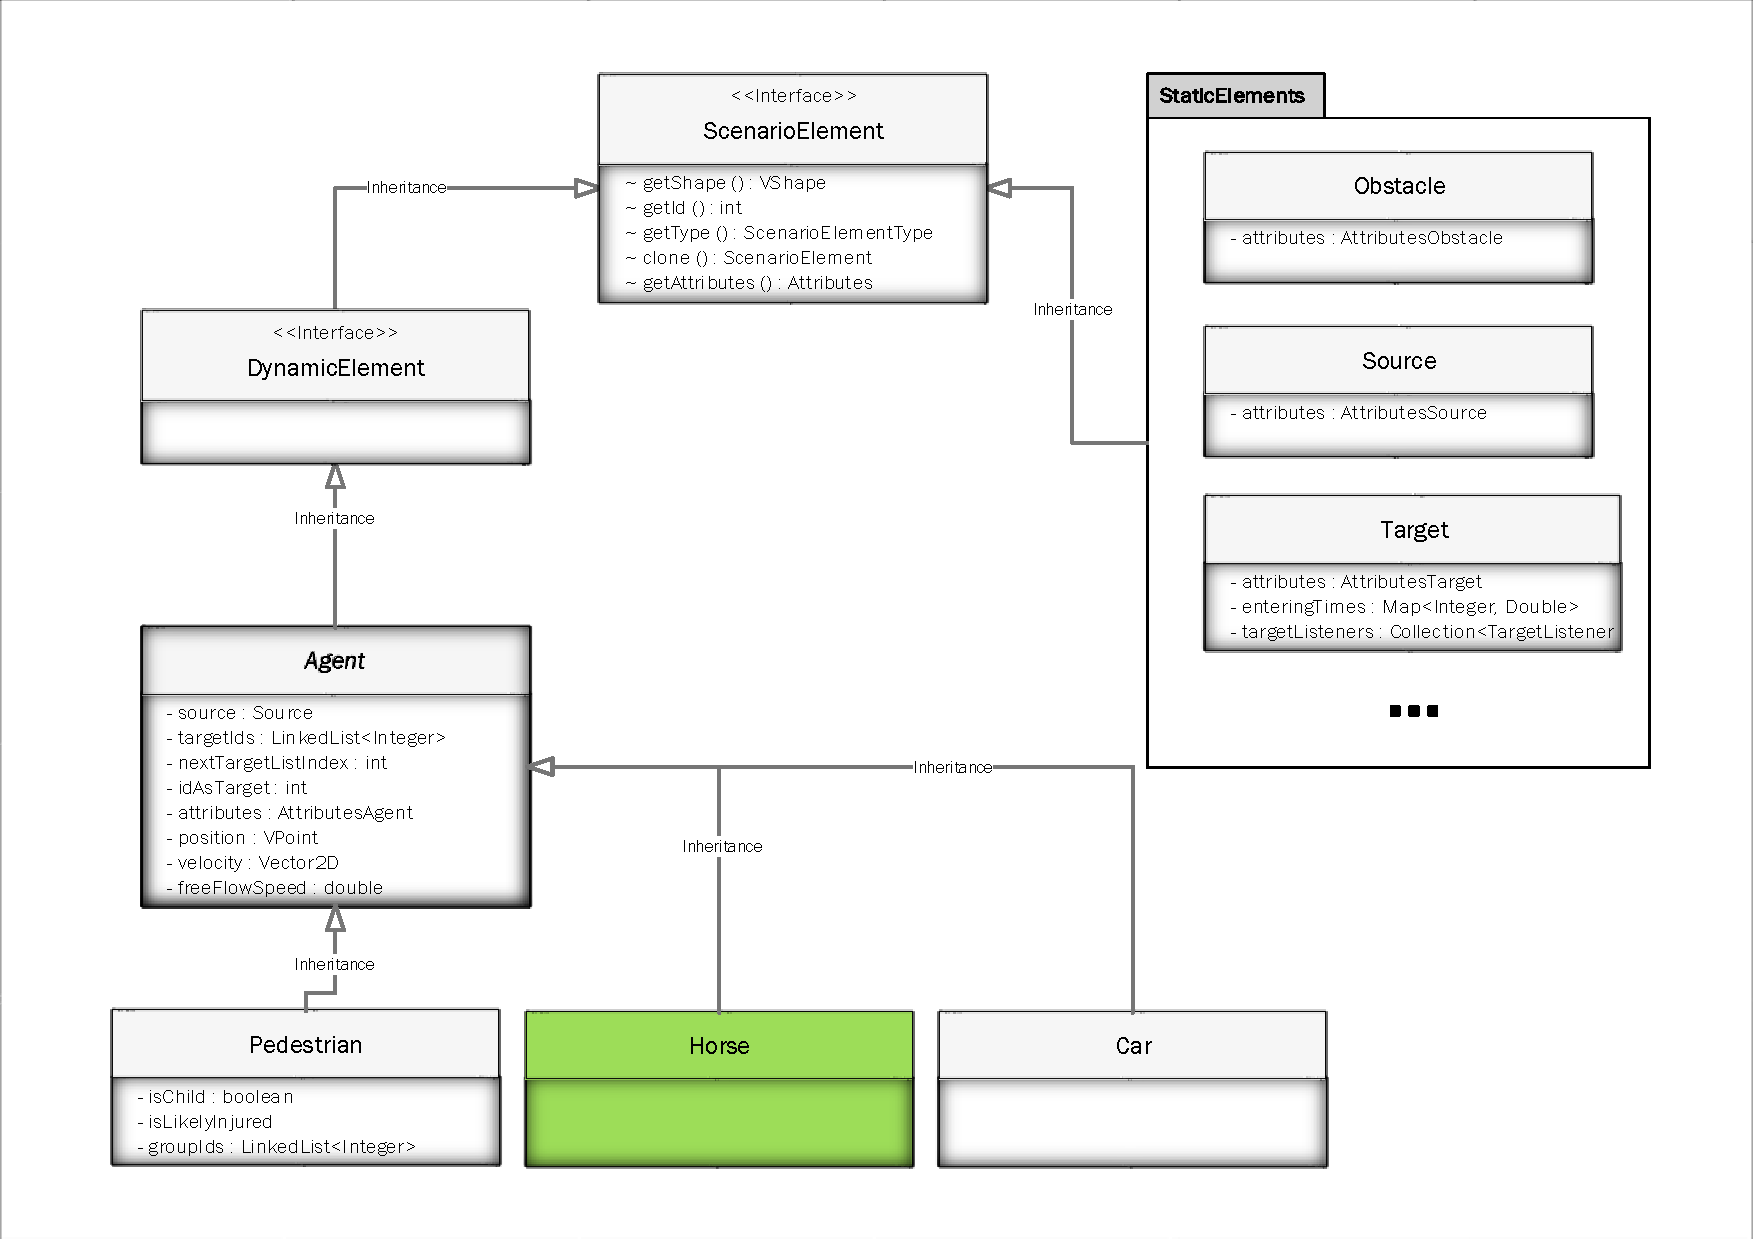
\includegraphics[width=\textwidth, keepaspectratio]{appendix/uml/ScenarioElements.pdf}
	\end{figure}
\end{frame}

\begin{frame}{Attribute}
	\begin{figure}
		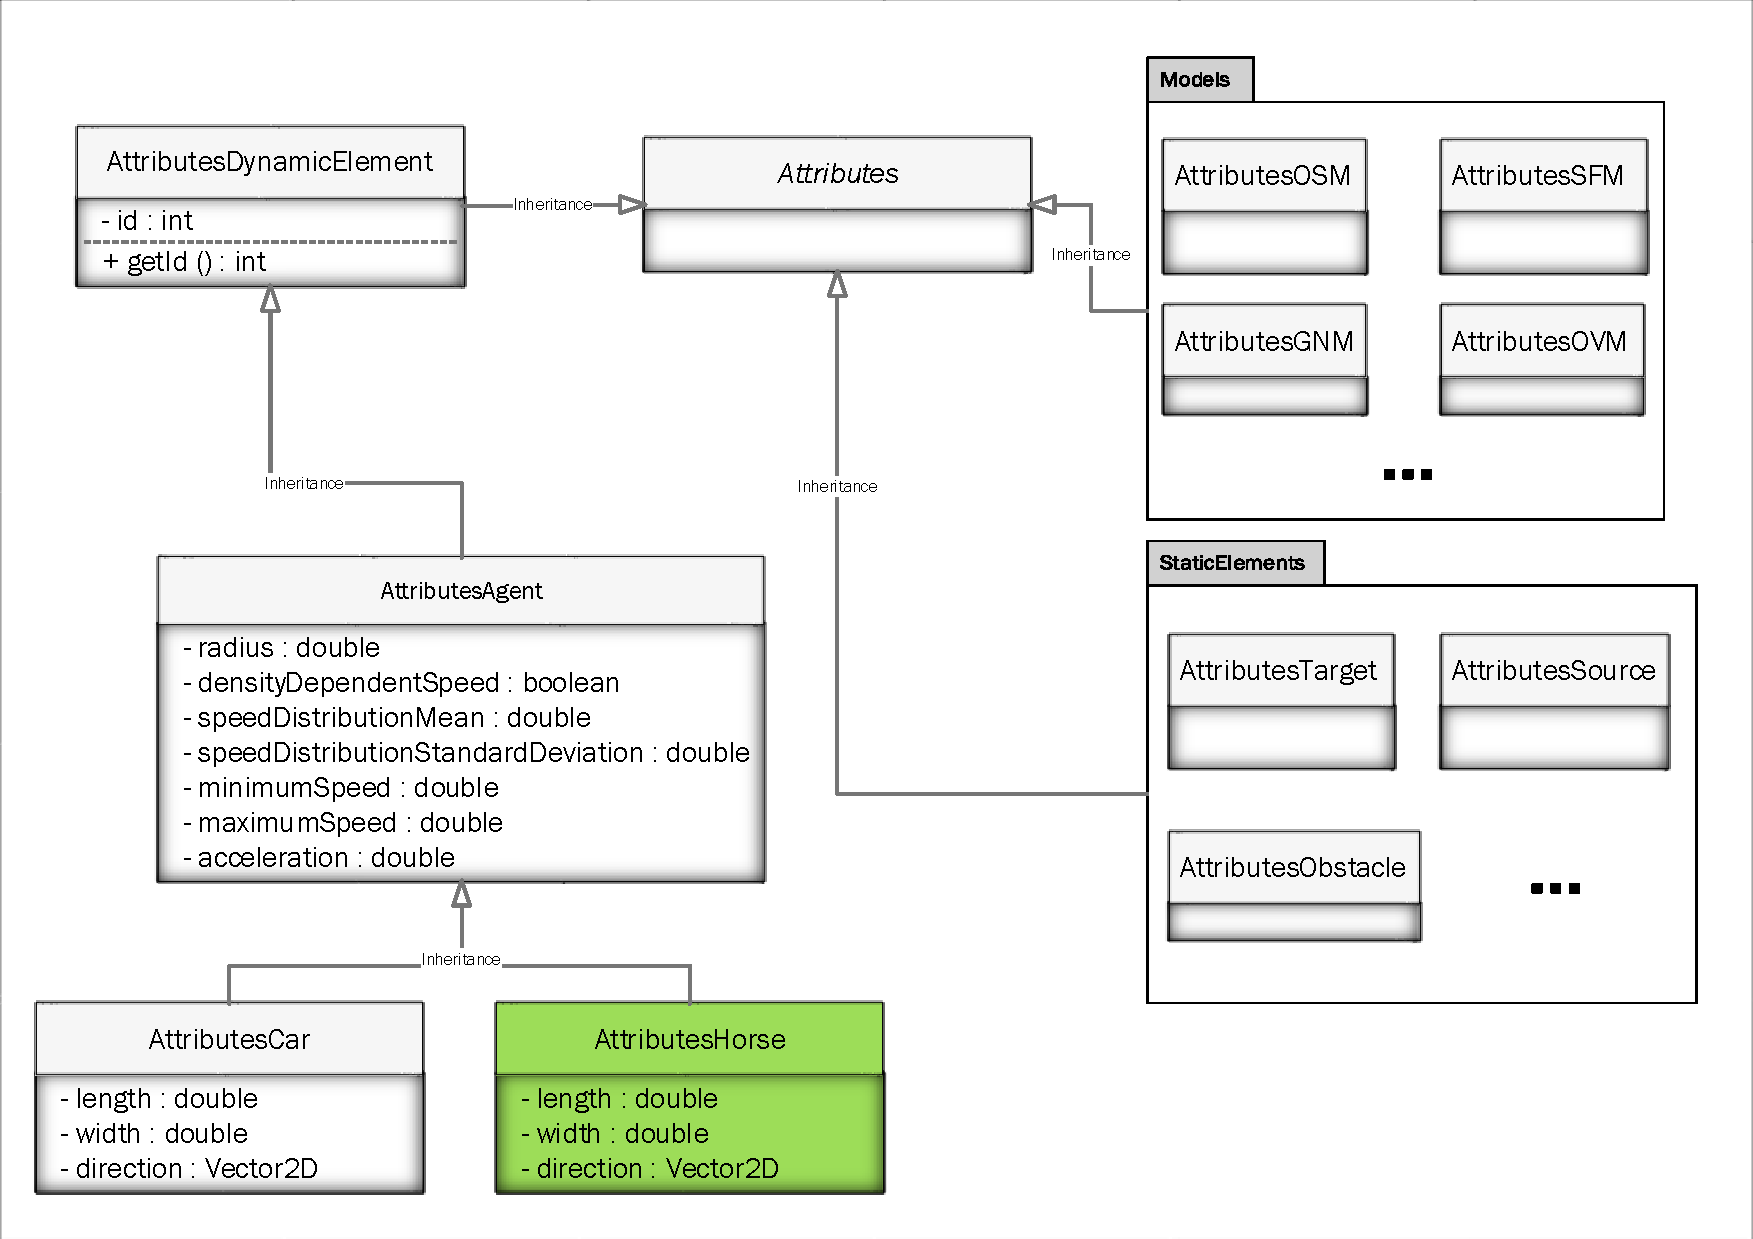
\includegraphics[width=\textwidth, keepaspectratio]{appendix/uml/Attributes.pdf}
	\end{figure}
\end{frame}

\begin{frame}{Ergebnisse}
	\begin{itemize}
		\item	Das Pferd kann in der Simulation, sowie in der GUI wie ein Fußgänger einbezogen werden
		\item Die Eigenschaften der Klassen Horse und AttributesHorse können serialisiert werden
	\end{itemize}
\end{frame}

\begin{frame}{Review: Arbeitsaufteilung}
	\begin{figure}
		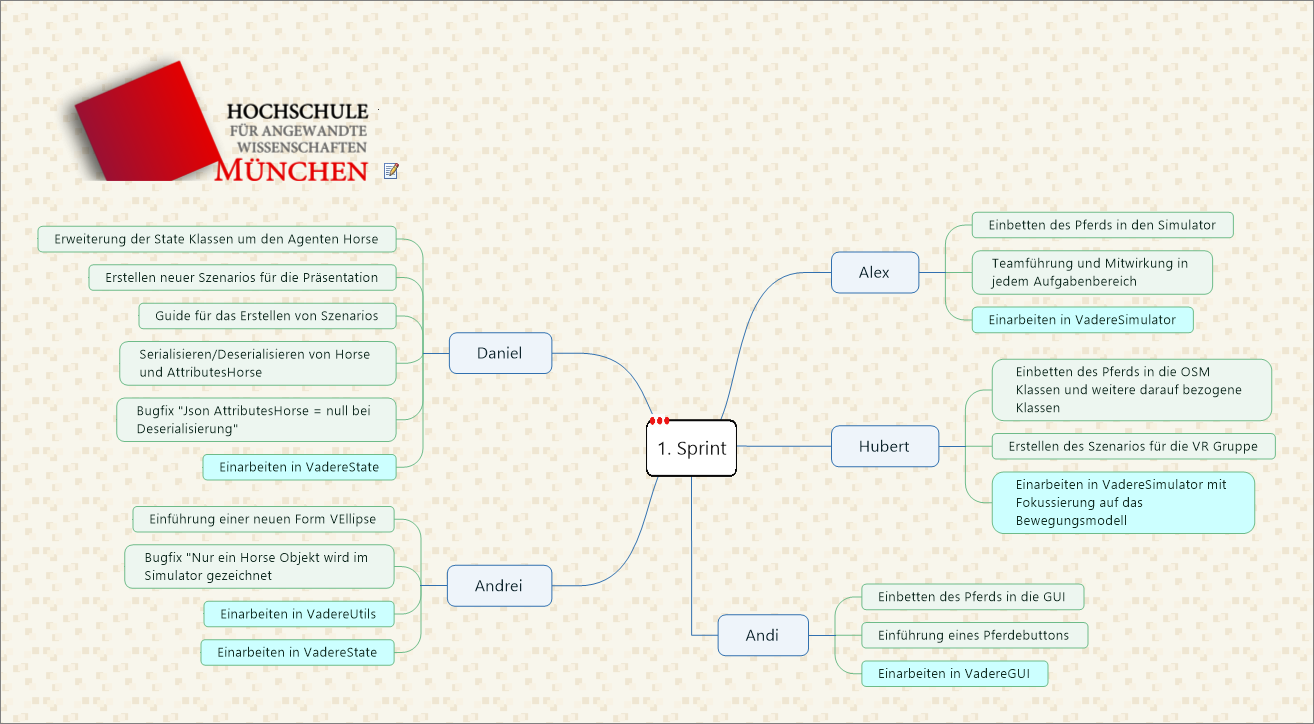
\includegraphics[width=\textwidth,keepaspectratio]{task_review.png}
	\end{figure}
\end{frame}
